%! suppress = MissingLabel

Как-то Joe Fasel в разговоре с Philip Wadler высказал идею того, что перегрузка функций (overloading) должна находить своё отражение в типах.
Wadler понял его неправильно~\cite{hudak2007history}.
Но то, что он понял, --- оказалось классами типов~\cite{wadler1989make}.

Christopher Strachey ввёл классификацию полиморфизма на две категории.
Параметрический --- один и тот же код работает с данными различных типов.
\vocab{Специальный (ad-hoc) полиморфизм} --- код выбирается в зависимости от типа.
Например, один и тот же символ умножения по-разному действует на целые числа и на числа с плавающей точкой.

Перегрузка в языках обозначает возможность назвать несколько функций одинаково, у которых должны быть различные наборы входных параметров.
В месте вызова компилятор статически определяет по типам аргументов, какую из них действительно следует вызвать.
\begin{minted}{cpp}
    string toString(x: int) { ... }
    string toString(fmt: String, d: double) { ... }
\end{minted}

Классы типов обязуют сначала задекларировать именованную сущность (собственно, класс типов), которая включает в себя пачку деклараций функций, которые могут быть перегружены для различных типов.
\begin{minted}{haskell}
    class Show a where
      show :: a -> String

    instance Show Int where
      show :: Int -> String
      show = ...
\end{minted}

Необходимо заметить, что декларация класса типов содержит формальный типовой параметр, по вхождениям которого в тип функции, собственно, выбирается перегрузка.
Таких параметров может быть много, они могут иметь стрелочные кайнды.
Например, в случае класса типов \mintinline{haskell}|Applicative|, выбор реализации операции \mintinline{haskell}|pure| будет происходить по типовому конструктору результата, то есть даже не по полноценному типу.
Такая гибкость и близко не достигается при классической перегрузке.
\begin{minted}{haskell}
    class Functor f => Applicative (f :: Type -> Type) where
      pure :: a -> f a
      ...

    instance Applicative Maybe where
      pure :: a -> Maybe a
      ...
\end{minted}

Также, в отличие от перегрузки, классы типов совместимы с параметрическим полиморфизмом.
Так, в типе полиморфной функции нельзя указать, что для типа должна присутствовать определённая перегрузка.
Классы типов же позволяют ограничить набор возможных типовых аргументов теми, для которых реализован инстанс нужного класса типов:
\begin{minted}{haskell}
    showPrefixed :: Show a => a -> String -> String
\end{minted}

Если сравнивать классы типов с переопределением (overriding) в ООП языках, то разрешение вызова виртуальной функции происходит с использованием таблицы, хранящейся объекте первого параметра (получателя вызова, receiver).
Классы типов же опираются исключительно на тип, поэтому, например, возможно определение констант в классах типов:
\begin{minted}{haskell}
    class Enum a => Bounded a where
      minBound :: a
      maxBound :: a
\end{minted}

В то же время, классы типов не являются типами, а, скорее, предикатами на типах.
Тип удовлетворяет такому предикату, или свойству, если для него есть соответствующий инстанс.
Поэтому, в частности, привычный способ в ООП создать гетерогенную коллекцию элементов, имеющих общий интерфейс, напрямую не сработает с классами типов.
Например, такой тип не будет корректным: \mintinline{haskell}|[Show]|.
Мы вернёмся к этой проблеме в~\ref{subsubsec:existentials}.

\subsection{Устройство классов типов}

Несмотря на поразительное могущество, идея реализации классов типов крайне проста.
Она была уже во всей полноте представлена в первой работе~\cite{wadler1989make}.
В дальнейших работах уточнялся механизм вывода типов в виде сведения к классической системе типов в стиле Hindley-Milner~\cite{hall1996type}.
Остальные работы, в основном, предлагают огромное разнообразие различных приложений.

\subsubsection{Словари}

Рассмотрим идею реализации классов типов на примере полиморфной сортировки.
Сортировка для списка элементов конкретного типа пишется тривиально:
\begin{minted}{haskell}
    sort :: [Int] -> [Int]
    sort = \case [] -> []; x:xs -> insert x (sort xs)
      where
        insert x xs = let (l, r) = List.partition (?\framebox{<}? x) xs in l ++ x : r)
\end{minted}

В реализации единственная информация о типе, которой мы пользуемся --- порядок на его обитателях.
Таким образом, при переходе к полиморфной сортировке, нам нужно принять словарь с предикатами, задающими нужный порядок для данного типа\footnote{Приятный синтаксис распаковки рекордов доступен с расширением \href{https://ghc.gitlab.haskell.org/ghc/doc/users_guide/exts/record_wildcards.html}{RecordWildCards}.}.
\begin{minted}{haskell}
    data OrdDict a = OrdDict { less :: a -> a -> Bool }

    sort :: OrdDict a -> [a] -> [a]
    sort d@OrdDict {..} = \case [] -> []; x:xs -> insert x (sort d xs)
      where
        insert x xs = let (l, r) = List.partition (?\framebox{`less`}? x) xs in l ++ x : r)
\end{minted}

Теперь, чтобы воспользоваться сортировкой на списке чисел, нужно сконструировать нужный рекорд и вызвать с ним функцию на списке конкретных типов:
\begin{minted}{haskell}
    intOrd :: OrdDict Int
    intOrd = OrdDict { less = (<) }

    ghci> sort intOrd [3, 2, 1]
\end{minted}

Возможна ситуация, когда инстанс для одного типа зависит от инстанса для другого
Например, сравнение списков можно получить автоматически, зная порядок на элементах.
В случае словарей мы это моделируем функцией между словарями:
\begin{minted}{haskell}
    listDict :: OrdDict a -> OrdDict [a]
    listDict d = OrdDict { less = ... ?\framebox{less d}? ... }
\end{minted}

Теперь мы можем сортировать список списков, конструируя нужный словарь:
\begin{minted}{haskell}
    ghci> sort (listDict intDict) [[3, 2], [2, 1], [0]]
\end{minted}

Сравнение явной передачи словарей и классов типов можно увидеть в следующей таблице:

\begin{tabular}{p{8cm}p{8cm}}
    \begin{enumerate}
        \item Определение словаря функций
        \begin{minted}{haskell}
            data MyOrd a = MyOrd
              { less :: a -> a -> Bool }
        \end{minted}
        \item Экземпляр словаря для конкретного типа
        \begin{itemize}
            \item Именованное значение
        \end{itemize}
        \begin{minted}{haskell}
            intMyOrd :: MyOrd Int
            intMyOrd = MyOrd { less = (<) }
        \end{minted}
        \item Явный параметр функции
        \begin{minted}{haskell}
            sort :: MyOrd a -> [a] -> [a]
        \end{minted}
        \item Передаётся пользователем
        \begin{minted}{haskell}
            test = sort ?\framebox{intMyOrd}? [3, 2, 1]
        \end{minted}
    \end{enumerate}
    &
    \begin{enumerate}
        \item Определение класса типов
        \begin{minted}{haskell}
             class MyOrd a where
               less :: a -> a -> Bool
        \end{minted}
        \item Объявление типа представителем класса типов
        \begin{itemize}
            \item Не имеет имени
        \end{itemize}
        \begin{minted}{haskell}
            instance MyOrd Int where
              less = (<)
        \end{minted}
        \item Неявный параметр функции
        \begin{minted}{haskell}
            sort :: MyOrd a => [a] -> [a]
        \end{minted}
        \item Передаётся компилятором
        \begin{minted}{haskell}
            test = sort [3, 2, 1]
        \end{minted}
    \end{enumerate}
\end{tabular}

Таким образом, словарь --- это свидетель (witness) того, что тип удовлетворяет ограничению.
Подобно тому, как коерции свидетельствуют несинтаксические эквивалентности на типах~\ref{subsubsec:gadts}.

\begin{task}
    Какой словарь будет соответствовать higher-kinded классу типов \mintinline{haskell}|Functor|?
\end{task}

\subsubsection{Неявные аргументы}

Можно думать так, что слева от \mintinline{haskell}|=>| передаются неявные аргументы функций, выводимые компилятором из контекста.
То есть, например, не стоит удивляться вхождениям \mintinline{haskell}|=>| в отрицательной позиции, это просто функция с неявным аргументом.
Так, следующий код не скомпилируется, потому что в месте использования переменной \texttt{y} нет значения типа \mintinline{haskell}|Show b|:
\begin{minted}{haskell}
    f :: (Show b => b) -> b
    f x = ?\framebox{x}?
\end{minted}
Можно это значение принять в функции \texttt{f}, тогда оно автоматически пропагируется в \texttt{y}:
\begin{minted}{haskell}
    f :: Show b => (Show b => b) -> b
    f x = ?\framebox{x}?
\end{minted}

Расширение \href{https://ghc.gitlab.haskell.org/ghc/doc/users_guide/exts/implicit_parameters.html}{ImplicitParams} даёт возможность делать некоторое аргументы функции неявными.
Фактически, это реализация динамического связывания в статическом языке~\cite{lewis2000implicit}.
Неявные аргументы берутся из скоупа по имени и подставляются автоматически:
\begin{minted}[escapeinside=##]{haskell}
    sortBy :: (a -> a -> Bool) -> [a] -> [a]

    sort :: (?cmp :: a -> a -> Bool) => [a] -> [a]
    sort = sortBy ?cmp
\end{minted}

Haskell также предоставляет возможность сохранять словари в структуры данных:
\begin{minted}{haskell}
    data ShowDict a where
      ShowDict :: Show a => ShowDict a

    f :: ShowDict b -> (Show b => b) -> b
    f d x = case d of ShowDict -> ?\framebox{x}? -- в скоупе доступен инстанс Show b
\end{minted}

\subsubsection{Вывод инстансов}

Чтобы вызвать ограниченно-полиморфную функцию, GHC производит вывод инстансов или, иначе говоря, автоматически конструирует свидетелей.
Вывод инстансов тесно интегрирован с общей системой вывода типов Haskell\footnote{\href{https://youtu.be/-TJGhGa04F8?si=vQDXYa3frYilXRhw}{(youtube) Type inference as constraint solving: how GHC’s type inference engine actually works - SPJ.}}.

В действительности вывод инстансов это не что иное, как \point{задача населения типа}.
Действительно, после трансляции в Core (промежуточное представление в GHC), классы типов представляют собой словари функций.
У нас в контексте имеются конкретные словари и функции, позволяющие из одних словарей получать другие.
Требуется найти терм, конструирующий словарь нужного типа.

Например, внутри функции \mintinline{haskell}|f :: Show a => ..| происходит вызов ограниченно- полиморфной функции
\mintinline{haskell}|g :: Show [a] -> ..|.
У нас имеется словарь \mintinline{haskell}|ShowDict a|, а так же функция \mintinline{haskell}|ShowDict a -> ShowDict [a]|, пришедшая из импортов\footnote{Инстансы можно импортировать пустым импортом: \mintinline{haskell}|import Module ()|.}.
Необходимо сконструировать терм типа \mintinline{haskell}|ShowDict [a]|.
Очевидно, это будет просто аппликации одного к другому.

Вывод инстансов происходит рекурсивно.
Чтобы вывести \mintinline{haskell}|ShowDict [a]|, выводится сначала посылка \mintinline{haskell}|ShowDict a|.
То есть получается рекурсия по структуре типа.
Иначе говоря, вывод инстансов можно эксплуатировать как вычислительный примитив уровня типов.
Так, например, мы можем опускать информацию из типов в термы:
\begin{minted}{haskell}
    type data Nat = Zero | Suc Nat

    class KnownNat (n :: Nat) where
      natVal :: Int

    instance KnownNat Zero where
      natVal = 0

    instance KnownNat n => KnownNat (Suc n) where
      natVal = 1 + natVal @n

    ghci> natVal @(Suc (Suc Zero))
    -- выведется natVal {knownSuc (knownSuc knownZero)}
\end{minted}

В общем случае процесс населения типа, как можно предположить по вычислительной аналогии, неразрешим.
Поэтому GHC накладывает большое количество ограничений на вид инстансов, которые гарантируют тотальность вывода.
Подробно эти ограничения описаны в~\cite{sulzmann2007understanding}.
Также GHC предоставляет различные расширения, ослабляющие эти ограничения и перекладывающие часть ответственности на плечи программиста\footnote{\url{https://downloads.haskell.org/ghc/latest/docs/users_guide/exts/instances.html}}.
Например, c UndecidableInstances можно легко написать разворот списка типов на этапе компиляции, как и любую другую функцию:
\begin{minted}{haskell}
    class Reverse (acc :: [Type]) (tys :: [Type]) where
      showReverse :: String

    instance ShowT acc => Reverse acc '[] where
      showReverse = showTypes @acc

    instance Reverse (ty : acc) tys => Reverse acc (ty : tys) where
      showReverse = showReverse @(ty : acc) @tys

    ghci> showReverse @'[] @'[Char, Int, Double]
\end{minted}

Вывод инстансов опирается только на вид "головы" декларации --- справа от \mintinline{haskell}|=>|, а ограничения слева применяются постфактум.
Это можно использовать, чтобы писать более общие инстансы.
Так, например, работает \vocab{constraint trick}\footnote{\url{https://chrisdone.com/posts/haskell-constraint-trick/}}, позволяющий резолвить ad-hoc полиморфные функции в параметрически-полиморфном контексте.

Этим же пользуется механизм программируемых ошибок компиляции из \href{https://hackage.haskell.org/package/base-4.20.0.1/docs/GHC-TypeLits.html}{GHC.TypeLits}.
Если инстанс сработал и компилятор начал обрабатывать ограничения слева, значит, что-то пошло не так~\cite[глава 12]{maguire-types}.

\begin{minted}{haskell}
    instance (TypeError
      ( Text "Attempting to show a function of type "
        :<>: Text "'" :<>: ShowType (a -> b) :<>: Text "'"
        :$$: Text "Did you forget to apply an argument?"
      )) => Show (a -> b) where
      show = undefined -- реализация не важна, до исполнения дело не дойдёт
\end{minted}

% todo lifting info to classes

\cite{kiselyov2004functional}

\subsubsection{Имплиситы и когерентность}

Существуют подходы к реализации классов типов, когда они не являются отдельной возможностью языка, а получаются как следствие других, более общих, механизмов.

Так, в Scala существует механизм имплиситов (implicits)~\cite{kvrikava2019scala}.
Параметры функции могут быть помечены \mintinline{scala}|implicit|.
Теперь, если в контексте есть \mintinline{scala}|implicit| значения и \mintinline{scala}|implicit| функции, аргументы сгенерируются автоматически исходя из типа параметра.
Теперь мы можем смоделировать словарь функций, например, с помощью интерфейсов (которые в Scala называются \mintinline{scala}|trait|) и синглтонов, чтобы получить вполне себе классы типов~\cite{oliveira2010type}.
Функции с имплисит-параметрами не являются в полном смысле функциями первого класса в Scala.
\begin{minted}{scala}
    trait Show[T] {
        def show(x: T): String
    }

    def show[T](x: T)(implicit ev: Show[T]): String = ev.show(x)

    implicit object intShow extends Show[Int] {
        def show(x: Int): String = x.toString
    }

    def showAll[T](xs: List[T])(implicit ev: Show[T]): String =
        xs.map(show(_)).join(", ")
\end{minted}

В языках с зависимыми типами неявные параметры\footnote{\url{https://agda.readthedocs.io/en/v2.7.0.1/language/implicit-arguments.html}} особенно нужны, потому что, например, типы --- это такие же параметры функции, как и все остальные.
Поэтому вывод типов~--- это фактически вывод неявных аргументов функций.
Более того, зависимые функции, вместе с аргументами часто принимают доказательства каких-то свойств этих аргументов, которые тоже хочется по возможности выводить из контекста автоматически.
В свете аналогии между классами типов как предикатами на типах, а инстансами как доказательствами, свидетельствующими о выполнении предиката для типа, можно тот же механизм вывода доказательств переиспользовать для эмулирования классов типов\footnote{\url{https://agda.readthedocs.io/en/v2.7.0.1/language/instance-arguments.html}}~\cite{devriese2011bright}.
В обратную сторону можно механизмы зависимой типизации эмулировать классами типов~\cite{mcbride2002faking}.

Выражение классов типов через другие механизмы может выглядеть как абсолютно выигрышная стратегия на фоне реализации их как самостоятельной возможности языка.
Действительно, можно переиспользовать всё то могущество программирования, которое есть с рекордами, в то время как для классов типов и констреинтов то же самое приходится развивать отдельно\footnote{\url{https://downloads.haskell.org/ghc/latest/docs/users_guide/exts/instances.html}}.
Да и неявные аргументы, наверное, полезный механизм сам по себе.

Однако у подхода Haskell есть важное свойство при соблюдении всех ограничений, т.е. при отсутствии \vocab{orphan instances}\footnote{\url{https://stackoverflow.com/questions/3079537/orphaned-instances-in-haskell}}.
\vocab{Когерентность инстансов (coherence)} --- для одного типа все инстансы данного класса типов, полученные разными способами, неотличимы (см.~\ref{fig:coherence}).
Соответственно, не имеет значения происхождение того или иного инстанса.
Иначе говоря, об этом можно не думать, это снимает существенное количество когнитивной нагрузки и упрощает рефакторинг\footnote{\href{https://youtu.be/hIZxTQP1ifo?si=aG2Lk2eb-5E5SOLb}{Edward Kmett - Type Classes vs. the World.}}.
В то время как остальные подходы требуют трепетного отношения к контексту вызова, потому что из него может прийти неожиданная реализация.

\begin{figure}
    \centering
    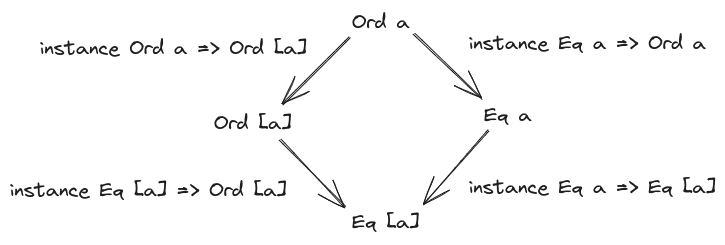
\includegraphics[width=0.8\linewidth]{figs/coherence}
    \caption{Когерентность инстансов --- диаграмма коммутирует.}
    \label{fig:coherence}
\end{figure}

\subsubsection{Правила (rules) и специализация}

% todo

\subsection{Семейства, ассоциированные семейства}

% todo fist-class type families

% todo \chapter*{FunWithTypeFuns}

% todo

\subsection{Кайнд Constraint}

\cite{constraint-kind}

% todo vadics example

% todo tuple constraints

% todo constraint families and constraint synonims

% todo https://downloads.haskell.org/ghc/latest/docs/users_guide/exts/quantified_constraints.html

% todo с constraint kinds фигня отсюда не нужна Haskell Type Constraints Unleashed

\cite{orchard2010haskell}

% todo

\subsection{Использование классов типов}

% todo

\subsubsection{Сериализация}

% todo

\subsubsection{Рефлексия на типах}

\cite{peyton2016reflection}

% todo

\subsubsection{Экзистенциальные типы} \label{subsubsec:existentials}

\cite[глава 7]{maguire-types}

% todo dynamic

% todo

\subsubsection{Получение значений с уровня типов}

% todo

\subsubsection{Коерции}

\cite{breitner2014safe}

\cite[глава 8]{maguire-types}

% todo type roles


% todo what do you want to give name to


% todo constraint is a proposition and dict is a proof

% todo constraints package of Edward Kmett

% todo monomorphism restriction

% todo pattern-matching on types

% todo serializer and serializable

% todo proxy

% todo algebra driven design

% todo rules and coersion

% todo type classes vs interfaces
% todo type classes via interfaces and implicits

% todo incoherent instances

% todo instance arguments

% todo Monoid a => Monad m ??

% todo https://downloads.haskell.org/ghc/latest/docs/users_guide/exts/constraints.html

% todo ConstraintKinds

% todo constraints and decidability

% todo https://chrisdone.com/posts/haskell-constraint-trick/

% todo A Reflection on Types SPJ paper

% todo haskell specialization

% todo https://wiki.haskell.org/Inlining_and_Specialisation

% todo existential types, different vtable implementations, value types support
% todo scala type classes
% todo type inhabitation, system FC, Symon's talk
% todo доклад SPJ
% todo open unions, data a la carte
% todo roles and coertions
% todo typeable & reflection
% todo reflecrtion https://www.tweag.io/blog/2017-12-21-reflection-tutorial/
% todo How to make ad-hoc polymorphism less ad-hoc

% todo C. V. Hall, K. Hammond, S. L. Peyton Jones, and P. L. Wadler. Type classes in haskell

% todo S. Peyton Jones, S. Weirich, R. A. Eisenberg, and D. Vytiniotis. A reflection on types. In A list of successes that can change the world,

% todo \chapter*{"Hackett: a metaprogrammable Haskell" by Alexis King}

% todo


% todo call stack

% todo примеры с HList

% todo orphans

Для GHC можно указать правила переписывания, которые заставят компилятор использовать специализированные версии для определённых типов\footnote{\href{https://downloads.haskell.org/~ghc/6.12.2/docs/html/users\_guide/rewrite-rules.html\#rule-spec}{GHC user guide. Rewrite rules. Specialization.}}.
\begin{minted}{haskell}
    {-# RULES "genericLookup/Int" genericLookup = intLookup #-}
\end{minted}

% todo functional dependencies & associated types

% todo https://downloads.haskell.org/~ghc/9.0.1/docs/html/users_guide/exts/constraints.html

% todo Orphan rules

% todo builder code serialization format from babylon

% todo associated type families

% todo reference dependent types

% todo рулесы, законы и оптимизация

% todo asking to fill parameters for you because they are very obvious. Implicit in dependently-typed languages

% todo variadics, open sums and products

% todo
